\documentclass{beamer}
\mode<presentation>
{
  \usetheme{Hannover}      % or try Darmstadt, Madrid, Warsaw, ...
  \usecolortheme{default} % or try albatross, beaver, crane, ...
  \usefonttheme{default}  % or try serif, structurebold, ...
  \setbeamertemplate{navigation symbols}{}
  \setbeamertemplate{caption}[numbered]
} 


\usepackage[english]{babel}
\usepackage[utf8x]{inputenc}
\usepackage{scrextend}
\usepackage{graphicx}
\usepackage{booktabs}
\usepackage{adjustbox}
\usepackage{marvosym}

\graphicspath{ {images/} }

\newcommand*{\Comb}[2]{{}^{#1}C_{#2}}%

\setbeamertemplate{footline}{
\hfill
\insertframenumber{}/
\inserttotalframenumber
}

\title[Pres]{Methods and Tools for the Analysis of Legacy Software Systems}
\author{Stana Adelina Diana}
\institute{Computer Science and Engineering Department\\
"Politehnica" University of Timisoara}
\date{2019}

\begin{document}

\begin{frame}
  \titlepage
\end{frame}

%%%%%%%%%%%%%%%%%%%%%%%%%%%%%%%%%%%%%%%%%%
\section{Presentation of the research topic}
 \begin{frame}
\frametitle{Presentation of the research topic}
 The thesis will develop methods for the analysis of software systems
 using historical information from the versioning systems\footnote{Versioning systems keep track of every change to a file over time so early versions can be restored and used by software teams.}. 
\end{frame}

%%%%%%%%%%%%%%%%%%%%%%%%%%%%%%%%%%%%%%%%%%
\section{State of the art in software dependencies}
 \begin{frame}
\frametitle{Structural dependencies}
\begin{block}{Definition}
Structural dependencies are the result of \it{source code analysis} and can be extracted from : members, call parameters, local variables. 
\end{block}

\begin{center}
     \begin{figure}
	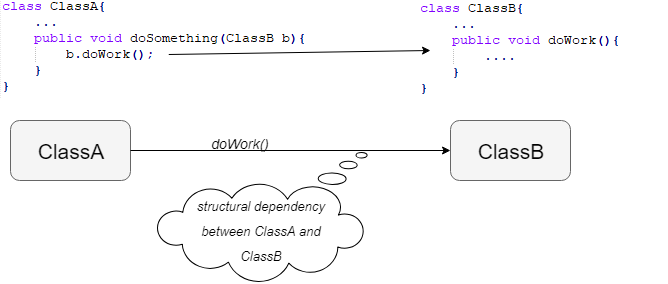
\includegraphics[width=\textwidth]{structural_dep.png}
	\caption{\label{fig:fig}Example of structural dependency between two classes}
     \end{figure}
\end{center}

\end{frame}

%%%%%%%%%%%%%%%%%%%%%%%%%%%%%%%%%%%%%%%%%%%

 \begin{frame}
\frametitle{Logical dependencies}
\begin{block}{Definition}
 Logical dependencies are the result of software history analysis and can reveal relationships that are not present in the source code code (structural dependencies).
\end{block}

\begin{center}
     \begin{figure}
	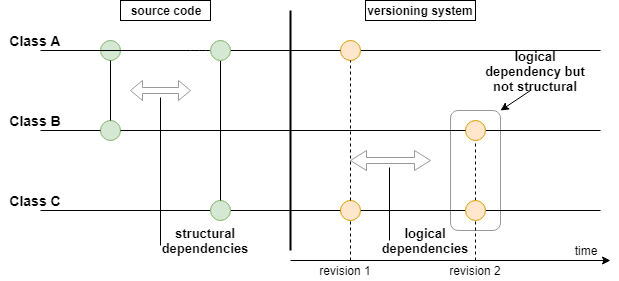
\includegraphics[width=\textwidth]{fig1.png}
	\caption{\label{fig:fig1}Example of logical and structural dependencies}
     \end{figure}
\end{center}

\end{frame}


%%%%%%%%%%%%%%%%%%%%%%%%%%%%%%%%%%%%%%%%%%%

 \begin{frame}
\frametitle{Applications of software dependencies}
\begin{itemize}
	\item Reverse engineering
	\item Architecture reconstruction
	\item Identifying clones
	\item Code smells
	\item Comprehension
	\item Fault location
	\item Error proneness
	\item Empirical software engineering research
\end{itemize}

\end{frame}

%%%%%%%%%%%%%%%%%%%%%%%%%%%%%%%%%%%%%%%%%%%

 \begin{frame}
\frametitle{Current status of research in identifying logical dependencies}
The current trend recommends that general dependency management methods and tools should also include logical dependencies besides the structural dependencies \footnote{Gustavo Ansaldi Oliva and Marco Aurelio Gerosa. On the interplay between
structural and logical dependencies in open-source software.} \footnote{Nemitari Ajienka and Andrea Capiluppi. Understanding the interplay between the logical and structural coupling of software classes.}. \\
But there are no strict rules to \textit{filter co-changes into logical dependencies}. Other researches filtered co-changes only in order to decrease their number and not to increase their validity.

\end{frame}


%%%%%%%%%%%%%%%%%%%%%%%%%%%%%%%%%%%%%%%%%%%
\section{Current status of doctoral research}
 \begin{frame}
\frametitle{Current status of doctoral research: Introduction}
We studied 20 open source systems written in Java and CSharp.
Filters and Thresholds:
\begin{itemize}
	\item commit size (cs): the maximum size of commit transactions
which are accepted to generate logical dependencies. The
values for this threshold were 5, 10, 20 and no threshold (infinity).
	\item  number of occurrences (occ): the minimum number of
repeated occurrences for a co-change to be counted as logical
dependency. The values for this threshold were 1, 2, 3 and 4.
	\item with/without taking comments into consideration as valid
change.
\end{itemize}


\end{frame}


%%%%%%%%%%%%%%%%%%%%%%%%%%%%%%%%%%%%%%%%%%%

\begin{frame}
\frametitle{Open source projects studied}
\vskip 0.2cm
\adjustbox{max height=\dimexpr\textheight-5.5cm\relax,
           max width=\textwidth}{
\begin{tabular}{*{5}{l}}
  \toprule
    ID  & Project    & Nr. of classes & Nr. of commits\\
    \midrule
1	&	urSQL	&	41	&	89	&	java	\\
2	&	JavaCoder	&	5	&	11	&	java	\\
3	&	jbandwidthlog	&	14	&	54	&	java	\\
4	&	sjava-logging	&	18	&	62	&	java	\\
5	&	daedalum	&	66	&	29	&	java	\\
6	&	prettyfaces	&	236	&	207	&	java	\\
7	&	jbal	&	102	&	113	&	java	\\
8	&	guavatools	&	237	&	85	&	java	\\
9	&	monome-pages	&	240	&	280	&	java	\\
10	&	kryo	&	309	&	743	&	java	\\
11	&	bitlyj	&	21	&	81	&	java	\\
12	&	slema	&	276	&	368	&	java	\\
13	&	bluecove	&	435	&	1679	&	java	\\
14	&	gp-net-radius	&	25	&	28	&	java	\\
15	&	aima-java	&	833	&	1181	&	java	\\
16	&	powermock	&	966	&	1512	&	java	\\
17	&	restfb	&	757	&	1545	&	java	\\
18	&	Tensorflow	&	1104	&	2386	&	cpp	\\
19	&	mangnum	&	143	&	1728	&	cpp	\\
    \bottomrule
  \end{tabular}}


\end{frame}

%%%%%%%%%%%%%%%%%%%%%%%%%%%%%%%%%%%%%%%%%%%

 \begin{frame}
\frametitle{Tool for measuring software dependencies}

\begin{center}
     \begin{figure}[H]
	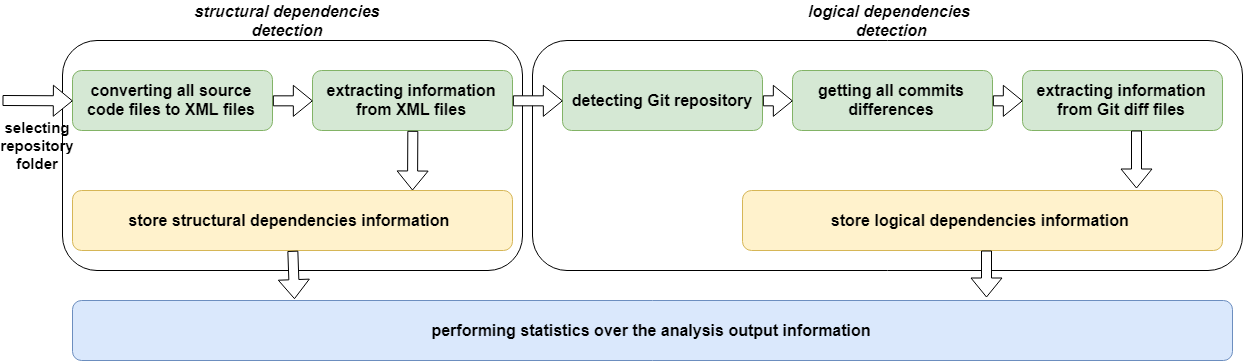
\includegraphics[width=\textwidth]{fig3.png}
	\caption{\label{fig:fig3}Workflow diagram of the tool}
     \end{figure}
\end{center}

\changefontsizes{7.5pt}
The workflow can be delimited by three major steps as it follows:
\begin{itemize}
\item Extracting structural dependencies.
\item Extracting co-changes.
\item Processing the information extracted.
\end{itemize}

\end{frame}

%%%%%%%%%%%%%%%%%%%%%%%%%%%%%%%%%%%%%%%%%%%

 \begin{frame}
\frametitle{Commit transactions size }
\vskip 0.2cm
\begin{center}
     \begin{figure}
	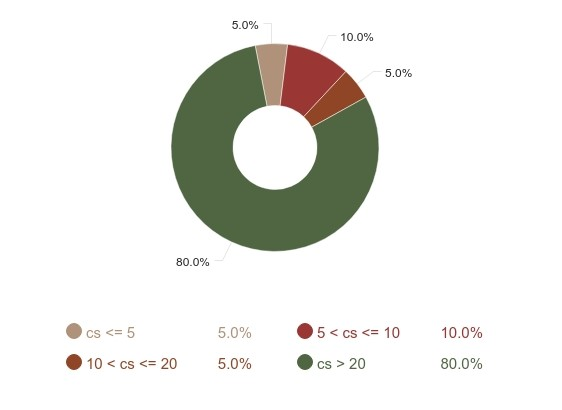
\includegraphics[width=\textwidth]{cs_size.jpg}
	\caption{\label{fig:fig4}Commit transactions size: overview in percentages}
     \end{figure}
\end{center}

\end{frame}


%%%%%%%%%%%%%%%%%%%%%%%%%%%%%%%%%%%%%%%%%%%

 \begin{frame}
\frametitle{Pairs of co-changes extracted }
\vskip 0.2cm
\begin{center}
     \begin{figure}
	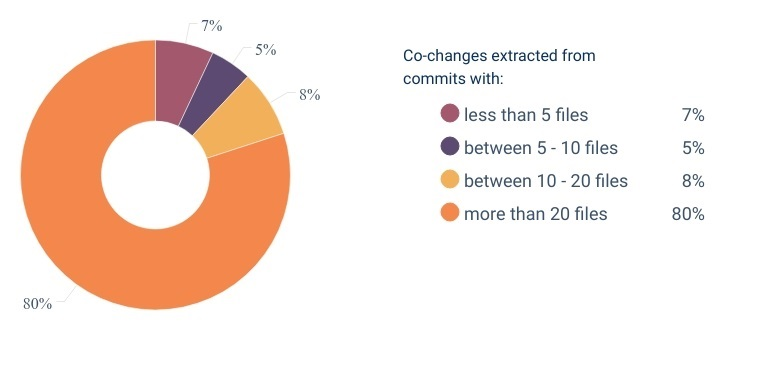
\includegraphics[width=\textwidth]{extracted_co.jpg}
	\caption{\label{fig:fig5}Pairs of co-changes extracted: overview in percentages}
     \end{figure}
\end{center}

\end{frame}

%%%%%%%%%%%%%%%%%%%%%%%%%%%%%%%%%%%%%%%%%%%

 \begin{frame}
\frametitle{Pairs of co-changes extracted - observation }
\vskip 0.2cm
\begin{center}
     \begin{figure}
	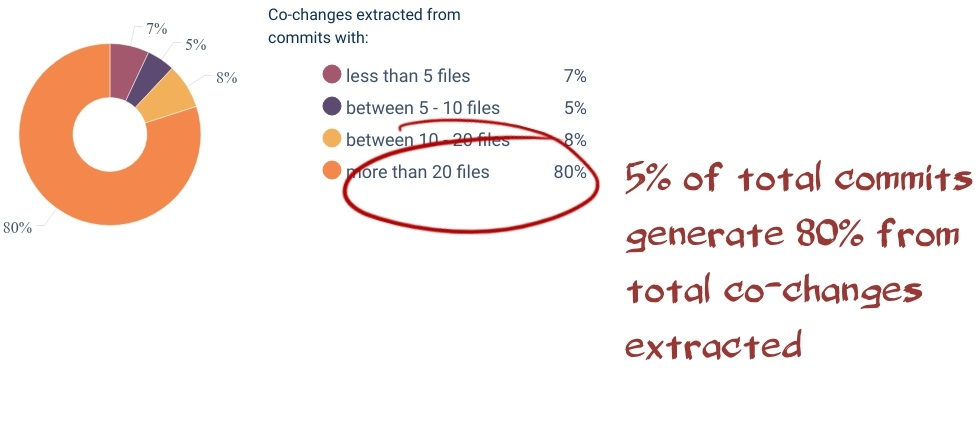
\includegraphics[width=\textwidth]{extracted_co2.jpg}
     \end{figure}
\end{center}

\end{frame}


%%%%%%%%%%%%%%%%%%%%%%%%%%%%%%%%%%%%%%%%%%%

 \begin{frame}
\frametitle{Comments changes}
\vskip 0.2cm
\begin{center}
     \begin{figure}
	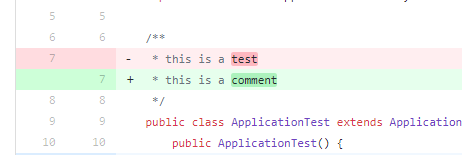
\includegraphics[width=\textwidth]{comment.PNG}
     \end{figure}
\end{center}
\vskip 0.4cm
\begin{itemize}
        \item approx -5\% from total co-changes extracted from all commit sizes
         \item approx -1\% from total co-changes extracted from commits with less than 10 files
\end{itemize}

\end{frame}

%%%%%%%%%%%%%%%%%%%%%%%%%%%%%%%%%%%%%%%%%%%

 \begin{frame}
\frametitle{Setting thresholds for the number of occurrences}
\vskip 0.2cm
\begin{center}
     \begin{figure}
	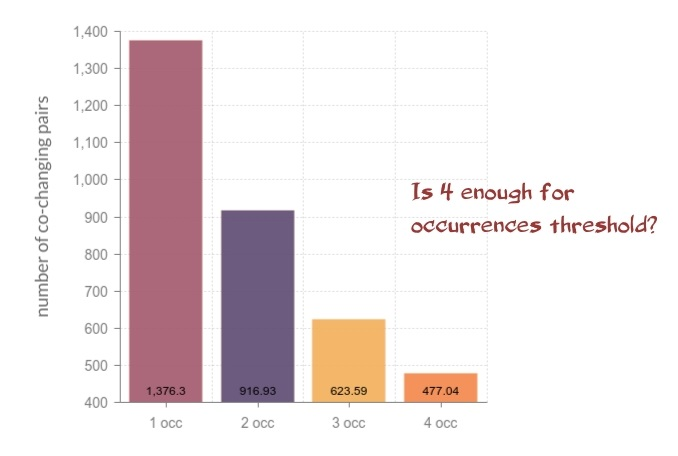
\includegraphics[width=\textwidth]{occ2.jpg}
	\caption{\label{fig:fig5}Pairs of co-changes extracted reported to occ threshold}
     \end{figure}
\end{center}
\end{frame}

%%%%%%%%%%%%%%%%%%%%%%%%%%%%%%%%%%%%%%%%%%%

 \begin{frame}
\frametitle{Refine filter for occurrences of co-changing classes}

\begin{center}
     \begin{figure}
	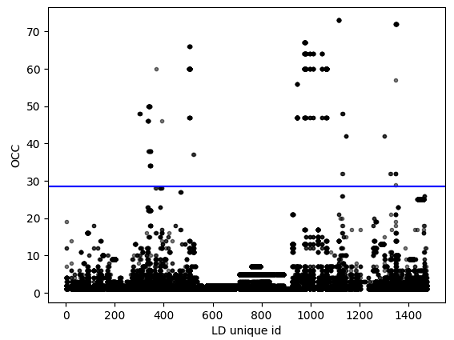
\includegraphics[width= 8.0 cm]{filter_occ.PNG}
	\caption{\label{fig:fig4} Occurrences rates of co-changing classes extracted from one system. Number of total commits: 6000. }
     \end{figure}
\end{center}

\end{frame}


%%%%%%%%%%%%%%%%%%%%%%%%%%%%%%%%%%%%%%%%%%%

 \begin{frame}
\frametitle{Logical and structural dependencies overlapping}
\vskip 0.2cm
\begin{center}
     \begin{figure}
	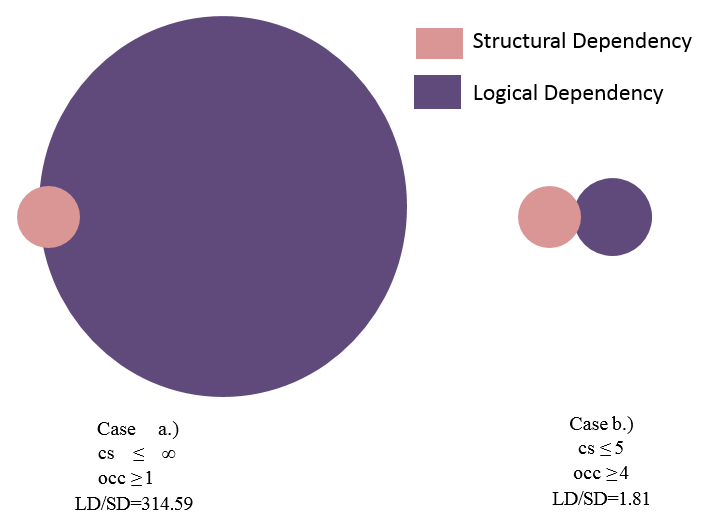
\includegraphics[width=\textwidth]{sd_vs_ld.PNG}
     \end{figure}
\end{center}
\end{frame}


%%%%%%%%%%%%%%%%%%%%%%%%%%%%%%%%%%%%%%%%%%


 \begin{frame}
\frametitle{Conclusions }
 \begin{itemize}
   	 \item The most important factors in co-changing classes filtering:
 \begin{itemize}
   	 \item  number of changed files taken into consideration (commit size)
	 \item number of occurrences 
    \end{itemize}
      	 \item Filtering thresholds shall be calculated according to the system size
     	 \item  + - 5\% for comment changes
    \end{itemize}

\end{frame}

%%%%%%%%%%%%%%%%%%%%%%%%%%%%%%%%%%%%%%%%%%%
\section{Research content and stages of research}
 \begin{frame}
\frametitle{Proposed research stages: Development of content and tools }

\textbf{Stage 1:} Build tool to extract structural dependencies from code and co-changes from git for a given set of projects.


\textbf{Stage 2:} Find filters for the co-changes extracted and establish different thresholds for those filters.


\textbf{Stage 3:} Study the impact of those filters and the corresponding thresholds on the remaining quantity of co-changes for each system.
Study the overlapping between the remaining pairs of co-changing entities and the structural dependencies extracted \footnote{Adelina Stana. and Ioana Sora. Identifying logical dependencies from
co-changing classes.  ENASE 2019.}  \footnote{Adelina Stana. and Ioana Sora. Analyzing information from versioning systems
to detect logical dependencies in software systems.  SACI 2019.}. 



\end{frame}

%%%%%%%%%%%%%%%%%%%%%%%%%%%%%%%%%%%%%%%%%%%

 \begin{frame}
\frametitle{Proposed research stages: Development of content and tools }

\textbf{Stage 4:} Establish a dynamic way to determine the thresholds for filters in order to fit the best each studied system. Main focus on the threshold for number of occurrences of co-changing pairs.
Use plots or other visual instruments in order to see the highest and the lowest rates for the numbers of occurrences among co-changing pairs.

\end{frame}

%%%%%%%%%%%%%%%%%%%%%%%%%%%%%%%%%%%%%%%%%%%

 \begin{frame}
\frametitle{Proposed research stages: Development of content and tools }

\textbf{Stage 5:} Take into account also structural dependencies from all the revisions of the system to filter out the old, out-of-date logical dependencies. Here an extra check is needed, it can be a case in which old structural dependencies that were also logically linked to continue to be logically linked
even after the structural dependency was removed.

\end{frame}

%%%%%%%%%%%%%%%%%%%%%%%%%%%%%%%%%%%%%%%%%%%

 \begin{frame}
\frametitle{Proposed research stages: Usage }

\textbf{Stage 6:} Use logical dependencies among structural dependencies in tools for architectural reconstruction to evaluate the improvement.

\textbf{Stage 7:} Compare the number of logical dependencies with metrics like Fan Out, Fan In and study their connections.
\begin{itemize}
	\item  Fan Out - number of other classes referenced by a class.
	\item  Fan In - number of other classes that reference a class.
\end{itemize}

\textbf{Stage 8:} Identify other tools that use structural dependencies and evaluate the impact of co-changes filtering into logical dependencies for them.

\end{frame}

%%%%%%%%%%%%%%%%%%%%%%%%%%%%%%%%%%%%%%%%%%%

 \begin{frame}
\frametitle{ Scientific reports and deadlines of stages}

\begin{figure}[H]
\centering
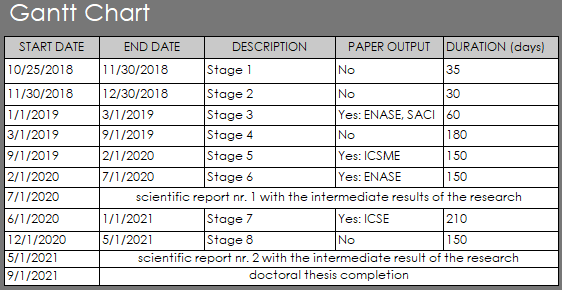
\includegraphics[width=\textwidth]{gantt_chart.PNG}
\label{fig:gantt1}
\end{figure}

\end{frame}


%%%%%%%%%%%%%%%%%%%%%%%%%%%%%%%%%%%%%%%%%%%

 \begin{frame}
\frametitle{Gantt chart}

\begin{figure}[H]
\centering
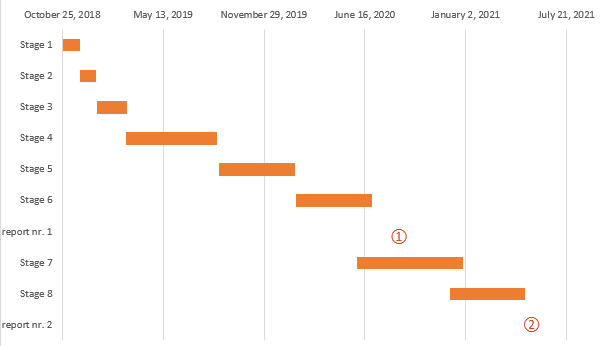
\includegraphics[width=\textwidth]{gantt_plot.PNG}
\label{fig:gantt2}
\end{figure}

\end{frame}


\end{document}